\iffalse
\chapter{2007}
\author{AI24BTECH11031}
\section{ae}
\fi

\item Across a normal shock
\begin{enumerate}
    \item both total temperature and total pressure decrease
    \item both total temperature and total pressure remain constant
    \item total pressure remains constant but total temperature decreases
    \item total temperature remains constant but total pressure decreases
\end{enumerate}

\item The Joukowskii airfoil is studied in aerodynamics because
\begin{enumerate}
    \item It is used in many aircraft
    \item It is easily transformed into a circle, mathematically
    \item It has a simple geometry
    \item It has the highest lift curve slope among all airfoils
\end{enumerate}

\item One of the criteria for high-speed airplanes is that the critical Mach number should
be as high as possible. Therefore, high-speed subsonic airplanes are usually designed with
\begin{multicols}{2}
    \begin{enumerate}
        \item thick airfoils
        \item thin airfoils
        \item laminar flow airfoils
        \item diamond airfoils
    \end{enumerate}
\end{multicols}

\item Two identical earth satellites $A$ and $B$ are in circular orbits at altitudes $h_A$
and $h_B$ above the earth's surface respectively, with $h_A > h_B$. If $E$ denotes the total
mechanical energy, $T$ the kinetic energy, and $V$ the gravitational potential energy of a
satellite, then:
\begin{multicols}{2}
    \begin{enumerate}
        \item $E_A > E_B$ and $V_A < V_B$
        \item $E_A > E_B$ and $T_A > T_B$
        \item $E_A < E_B$ and $T_A > T_B$
        \item $E_A > E_B$ and $T_A < T_B$
    \end{enumerate}
\end{multicols}

\item Let $\vec{P}$ and $\vec{Q}$ be two square matrices of the same size. Consider the following statements:
\begin{enumerate}[label=(\roman*)]
    \item $\vec{PQ} = \vec{0}$ implies $\vec{P} = \vec{0}$ or $\vec{Q} = \vec{0}$ or both
    \item $\vec{PQ} = \vec{I}$ implies $\vec{P} = \vec{Q}^{-1}$
    \item $\brak{\vec{P} + \vec{Q}}^2 = \vec{P}^2 + 2\vec{PQ} + \vec{Q}^2$
    \item $\brak{\vec{P} - \vec{Q}}^2 = \vec{P}^2 - 2\vec{PQ} + \vec{Q}^2$
\end{enumerate}
where $\vec{I}$ is the identity matrix. Which of the following statements is correct?
\begin{enumerate}
    \item (i), (ii) and (iii) are false, but (iv) is true
    \item (i), (ii) and (iv) are false, but (iii) is true
    \item (ii), (iii) and (iv) are false, but (i) is true
    \item (i), (iii) and (iv) are false, but (ii) is true
\end{enumerate}

\item A $1 kg$ mass attached to a spring elongates it by $16 mm$. The mass is then pulled from its
equilibrium position by $10 mm$ and released from rest. Assuming the acceleration due to gravity
of $9.81 m/s^2$, the response of the mass in mm is given by:
\begin{multicols}{2}
    \begin{enumerate}
        \item $x = 10 \cos 24.76t$
        \item $x = 10 \cos 24.76t$
        \item $x = \sin 16t$
        \item $x = 10 \cos 16t$
    \end{enumerate}
\end{multicols}

\item The earth's radius is $6.37 \times 10^6$ m and the acceleration due to gravity on its surface
is $9.81 m/s^2$. A satellite is in a circular orbit at a height of $6.30 \times 10^6$ m above the
earth's surface. The minimum additional speed it needs to escape from the earth's gravitational field is:
\begin{multicols}{2}
    \begin{enumerate}
        \item $3.66 \times 10^3 m/s$
        \item $3.12 \times 10^3 m/s$
        \item $3.27 \times 10^3 m/s$
        \item $3.43 \times 10^3 m/s$
    \end{enumerate}
\end{multicols}

\item Shown in the figure below is a model of a Euler-Bernoulli beam made up of two
materials subjected to pure bending moment $M$. The Young's modulus of material $A$
and $B$ are $E_A$ and $E_B$ respectively. The sectional moment of area about the neutral
axis of the cross-sectional area made of materials $A$ and $B$ are $I_A$ and $I_B$
respectively. The radius of curvatures $\rho$ of the flexural deflection of
this composite beam to the bending moment $M$ is then

\begin{center}    
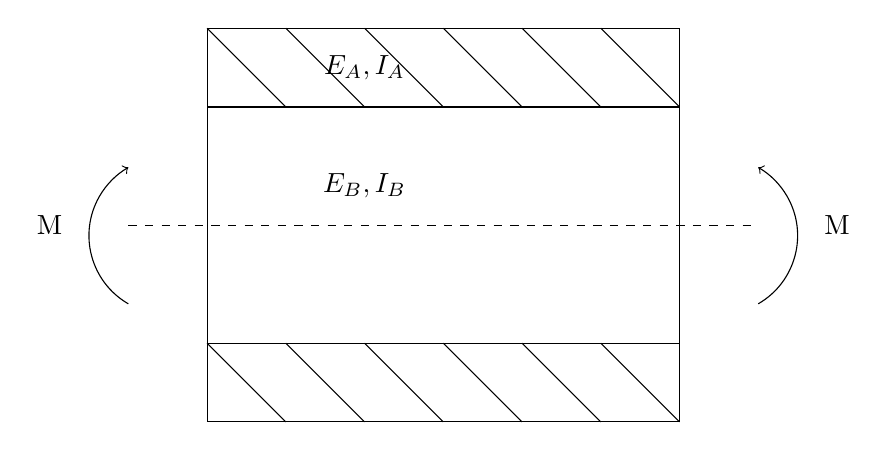
\begin{tikzpicture}
    \draw (-1,-1) rectangle (5,4);
    \foreach \i in {-1,...,4} {
        \draw (\i,4) -- (\i+1,3);
    }
    \foreach \i in {-1,...,4} {
        \draw (\i,0) -- (\i+1,-1);
    }
    \draw (-1, 3) -- (5, 3);
    \draw (-1, 0) -- (5, 0);
    \draw[dashed] (-2,1.5) -- (6,1.5);
    \draw[->] (6,0.5) arc[start angle=-60, end angle=60, radius=1cm];
    \draw[->] (-2,0.5) arc[start angle=240, end angle=120, radius=1cm];
    \node at (1, 2) {$E_B,I_B$};
    \node at (1, 3.5) {$E_A,I_A$};
    \node at (-3, 1.5) {M};
    \node at (7, 1.5) {M}; 
\end{tikzpicture}
\end{center}

\begin{multicols}{4}
    \begin{enumerate}
        \item $\rho = \frac{E_AI_A + E_BI_B}{M}$
        \item $\rho = \frac{E_AI_B + E_BI_A}{M}$
        \item $\rho = \frac{M}{E_AI_A + E_BI_B}$
        \item $\rho = \frac{\brak{E_A + E_B}\brak{I_A + I_B}}{M}$
    \end{enumerate}
\end{multicols}

\item Two pipes of constant sections but different diameters carry water
at the same volume flow rate. The Reynolds number, based on the pipe diameter, is


\begin{multicols}{2}
    \begin{enumerate}
        \item the same in both pipes
        \item is larger in the narrower pipe
        \item is smaller in the narrower pipe
        \item depends on the material of the pipes
    \end{enumerate}
\end{multicols}

\item Two airfoils of the same family are operating at the same angle of attack. The
dimensions of one airfoil are twice as large as the other one. The ratio of the
minimum pressure coefficient of the larger airfoil to the minimum pressure coefficient
of the smaller airfoil is

\begin{multicols}{4}
    \begin{enumerate}
        \item 4.0
        \item 2.0
        \item 1.0
        \item 0.5
    \end{enumerate}
\end{multicols}

\item Wing $A$ has a constant chord $c$ and span $b$. Wing $B$ is identical but has a span
$4b$. When both wings are operating at the same geometric angle of attack at subsonic speed, then

\begin{enumerate}
    \item wings A and B produce the same lift coefficient
    \item wing A produces a smaller lift coefficient than wing B
    \item wing A produces a greater lift coefficient than wing B
    \item the freestream Mach number decides which wing produces the greater lift coefficient
\end{enumerate}

\item A spring-mass damper system is excited by a force $F_0\sin\omega t$. The amplitude at resonance
is measured to be $1 cm$. At half the resonant frequency, the amplitude is $0.5 cm$. The damping ratio
of the system is

\begin{multicols}{4}
    \begin{enumerate}
        \item 0.1026
        \item 0.3242
        \item 0.7211
        \item 0.1936
    \end{enumerate}
\end{multicols}

\item The eigenvalues of the matrix $\vec{A} = \myvec{2 & 1 \\ 0 & 3}$ are

\begin{multicols}{4}
    \begin{enumerate}
        \item 1 and $\frac{1}{2}$
        \item 1 and $\frac{1}{3}$
        \item 2 and 3
        \item $\frac{1}{2}$ and $\frac{1}{3}$
    \end{enumerate}
\end{multicols}

\item The eigenvalues of the matrix $\vec{A}^{-1}$, where $\vec{A} = \myvec{2 & 1 \\ 0 & 3}$ are

\begin{multicols}{4}
    \begin{enumerate}
        \item 1 and $\frac{1}{2}$
        \item 1 and $\frac{1}{3}$
        \item 2 and 3
        \item $\frac{1}{2}$ and $\frac{1}{3}$
    \end{enumerate}
\end{multicols}

\item The radius of the earth is $6.37 \times 10^6 m$ and the acceleration due to gravity
at its surface is $9.81 m/s^2$. A satellite is in circular orbit at a height of
$35.9 \times 10^6 m$ above the earth's surface. The orbit is inclined at 10.5 degrees to
equator. The velocity change needed to make the orbit equatorial is:

\begin{enumerate}
    \item $561 m/s$ at $84.75$ degrees to the initial direction
    \item $561 m/s$ at $95.25$ degrees to the initial direction
    \item $281 m/s$ at $84.75$ degrees to the initial direction
    \item $281 m/s$ at $95.25$ degrees to the initial direction
\end{enumerate}

\item A piston-prop airplane having propeller efficiency $\eta_P = 0.8$ and weighing $73108 N$
could achieve maximum climb of $15 m/s$ at flight speed of $50 m/s$. The excess Brake Power (BP)
at the above flight condition will be

\begin{multicols}{4}
    \begin{enumerate}
        \item $1700 kW$
        \item $2100 kW$
        \item $1371 kW$
        \item $6125 kW$
    \end{enumerate}
\end{multicols}

\item An airplane model with a symmetric airfoil was tested in a wind tunnel $C_{m0}$ $\brak{C_m\text{ with
angle of attack, }\alpha = 0}$ was estimated to be $0.08$ and $0$ respectively for elevator settings
$\brak{\delta e}$ of 5 degrees up and 5 degrees down. The estimated value of the elevator control power
$\brak{\frac{\partial C_m}{\partial \delta e}}$ of the model will be

\begin{multicols}{2}
    \begin{enumerate}
        \item 0.07 per deg
        \item -1.065 per deg
        \item -0.008 per deg
        \item -0.762 per deg
    \end{enumerate}
\end{multicols}
